\newpage
\section{AWS IoT Greengrass}
\gls{AWS} Greengrass consists of a cloud part running in the \gls{AWS} data centers around the world and a local part which runs on e.g. self owned hardware like a Raspberry Pi \cite{AmazonWebServicesHowItWorks}. It's important to note there are two versions of AWS IoT Greengrass and only version two (v2) is discussed here. Version two is the newer one and isn't compatible with the API's from version one \cite{aws-greengrass-guide}. Figure \ref{fig:aws-greengrass-how-it-works} shows the two parts of Greengrass and the connections between them. The core devices are the edge devices which act locally on generated data to e.g. run predictions, aggregation tasks and more. These tasks can be bundled inside so-called components, which then can be deployed to the Greengrass core devices. Supported component runtimes are AWS Lambda functions, Docker containers, native OS processes, or custom runtimes. \cite{AmazonWebServicesHowItWorks}. Some runtimes like Docker or Python are not installed by the Greengrass installer and have to be installed manually by the developer or script, if the use is desired. The cloud part consists of the AWS IoT Greengrass cloud service which manages the core devices and any other AWS service which can be used by the core devices.

\begin{figure}[H]
    \centering
    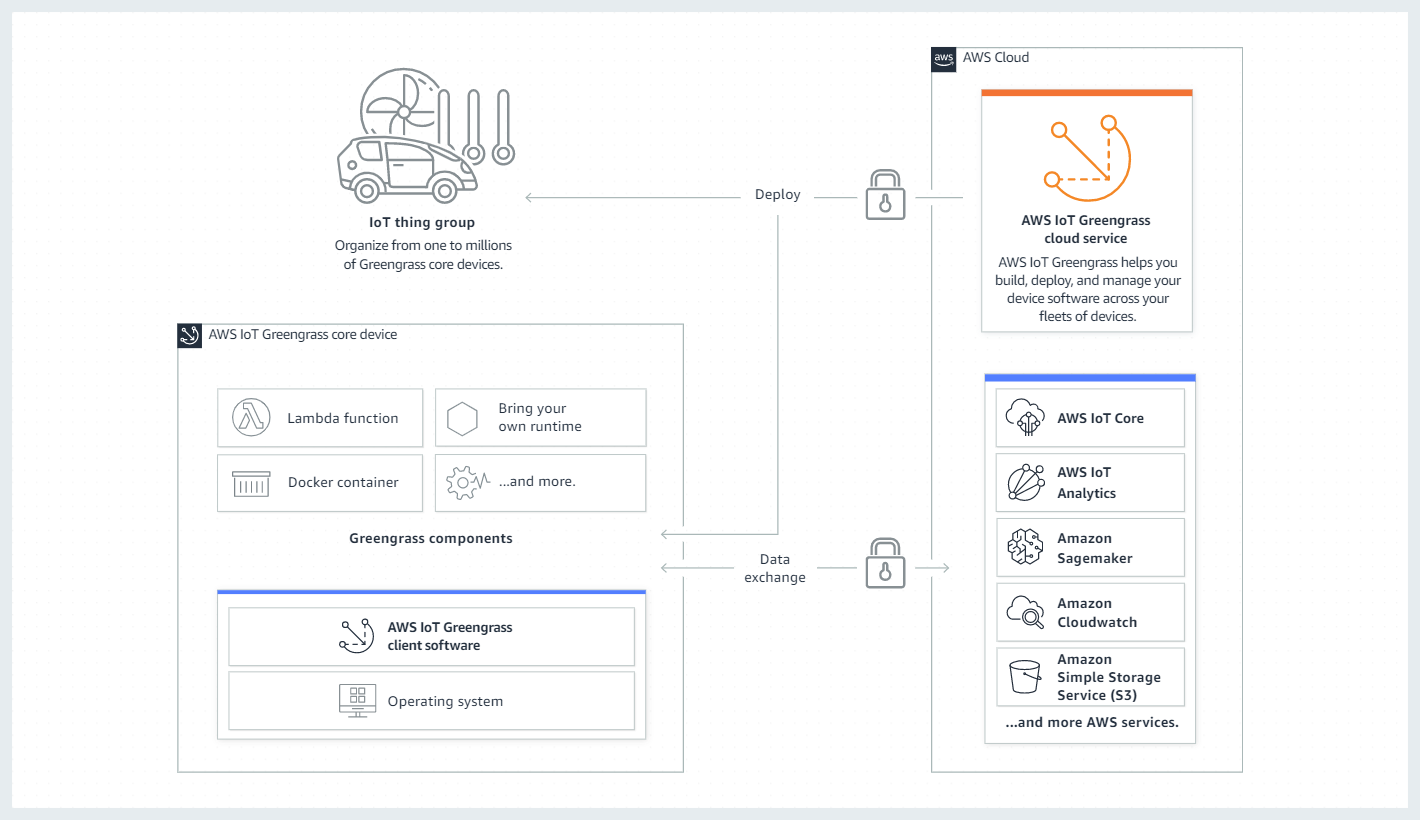
\includegraphics[width=\textwidth]{assets/aws-greengrass/aws-greengrass-how-it-works.png}
    \caption{AWS IoT Greengrass Architecture \cite{AmazonWebServicesHowItWorks}.}\label{fig:aws-greengrass-how-it-works}
\end{figure}

\paragraph{Greengrass core device:}
The core device is the device where edge computing ultimately takes place by running various components in different runtimes. Nearly everything can be deployed to the core device, like the \gls{AWS} Greengrass intro already mentions. For example, the core device contains an AWS provided MQTT broker which provides an interface for local IoT devices and allows them to directly publish and subscribe to the core device. The published messages can then be further processed by custom components directly on the core device \cite{AmazonWebServicesHowItWorks}.

\paragraph{Greengrass component:} Components are a software module that is deployed to the core device. This software module contains the executable software. Pre-built public components like the MQTT broker or log manager are provided by \gls{AWS}.
\cite{AmazonWebServicesHowItWorks}

\paragraph{Greengrass client device:} Client devices are the sensors/actors or generally the devices which connect to the core device for exchanging messages. Client devices do not need to know the direct address of the core device but can request it by means of a discovery process \cite{AmazonWebServicesHowItWorks}.

\paragraph{Greengrass cloud service:} The Greengrass cloud service is the cloud part which allows the developer to manage all the core devices and the distribution of Greengrass components \cite{AmazonWebServicesHowItWorks}.

\newpage
\subsection{Use case implementation}
The figure \ref{fig:aws-ggc-arch} below shows the implemented architecture and all the used components for the use case implementation. On the cloud side no services except the necessary ones were used. Inside the Greengrass core device the components are divided into AWS provided components and custom self written components. The MQTT protocol is used for communication between the cloud service and the core device. The client devices like the BMP280 and MQ2 sensor also use the \gls{MQTT} protocol to communicate with the core device. How the services on the core device were implemented will be explained in the following sections.

\begin{figure}[H]
    \fontsize{7}{10}\selectfont
    \centering
    \def\svgwidth{\textwidth}
    \input{assets/aws-greengrass/aws-greengrass-arch.drawio.pdf_tex}
    \caption{AWS Greengrass architecture overview.}
    \label{fig:aws-ggc-arch}
\end{figure}

\subsubsection*{Node setup}\label{subsubsec:aws-ggc-devices}
All three nodes were provisioned with the Ansible\footnote{\url{https://www.ansible.com/}} tool. The self written Ansible playbook follows the \gls{AWS} developer guide\footnote{\url{https://docs.aws.amazon.com/greengrass/v2/developerguide/quick-installation.html}} of installing the Greengrass Core with the \gls{AWS} provided installer. Besides the basic setup, which is explained in the developer guide, additional tools like Docker and Python get installed too. Before running the Ansible playbook against the configured devices the tool Terraform creates some \gls{AWS} resource like the device role, S3 bucket for storing artifacts and \gls{AWS} \gls{ECR} for storing private container images. After the Greengrass Core is installed on all configured devices, they will show up in the \gls{AWS} console under the Greengrass section in IoT Core. The devices contain only the basic components after the initial installation. By configuring the discovery feature for client devices, the \gls{AWS} provided components from figure \ref{fig:aws-ggc-arch} get installed on each core device of the same \textit{Thing group}. This discovery feature enables client devices to find and connect to discovered core devices. All devices which were set up from the example Ansible playbook are of the same \textit{Thing group}. The components get installed by creating and then triggering a deployment to the devices. Two of the components need configuring before deploying. The Auth component requires a JSON which describes which client devices are allowed to connect to the Greengrass Core device. The \gls{MQTT} bridge component also requires a JSON which describes the relaying of received and published messages. Example configuration JSON files can be found in the attached Git repository.

\newpage
\subsubsection*{Client devices}
All three devices BMP280, MQ2 and Ventilator need adjustments to connect to a Greengrass Core Device. At first, each new device needs to be registered as a \textit{thing} in the AWS Console. By registering the device, AWS allows the recommended certificate and key generation. This will generate a certificate and a public/private RSA key pair which is unique to each device. These certificates and keys are then used to authenticate the device against AWS and the Greengrass Core device. By registering a device, there is also the option of a \textit{policy}, which can be attached individually to each device. This policy provides information about what a device may or may not allowed to do. For this implementation the policy looks like the JSON in listing \ref{lst:iot-device-policy}. The policy in listing \ref{lst:iot-device-policy} allows the sensors and actors to connect, publish, subscribe and receive messages from the AWS IoT \gls{MQTT} broker. In addition to the \gls{MQTT} actions, the Greengrass action allows the device to discover local Greengrass core devices. Like the \textit{"Node Setup"} section in \ref{subsubsec:aws-ggc-devices} already mentions, the discovery feature must be enabled and configured before IoT device can connect to a local core device. Also, IoT devices must be manually added to the client devices list on each Greengrass core device to be able to discover the corresponding core device.

\begin{lstlisting}[caption={Client device policy.},label={lst:iot-device-policy},captionpos=b]
{
  "Version": "2012-10-17",
  "Statement": [
    {
      "Effect": "Allow",
      "Action": [
        "iot:Connect",
        "iot:Publish",
        "iot:Subscribe",
        "iot:Receive",
        "greengrass:*",
      ],
      "Resource": "arn:aws:iot:<region>:<account_id>:*"
    }
  ]
}
\end{lstlisting}

\subsubsection*{MQTT}
The communication with client devices works with an integrated MQTT broker. In addition to the MQTT broker is the MQTT bridge which is responsible to map MQTT messages to different messaging technologies. In total there are three different messaging technologies which cane be utilized by the Greengrass core devices. The first is the already mentioned MQTT broker, which provides the ability to publish and subscribe to specific MQTT topics. The second one is the \textit{PubSub} broker for local, device internal, publishing and subscribing. Local components can subscribe and publish to the PubSub broker by using \gls{IPC}. The third and the last one is the \textit{IoT Core} which simply transfers configured topics to the AWS IoT Core in the cloud for further use by e.g. \gls{AWS} cloud services. This option requires internet connection. Connection loses are ok due to the integrated queue, which will send the messages again after reconnect \cite{AmazonWebServicesMQTTBridge}. The MQTT bridge allows the developer to configure the mapping from one messaging technology to another. This configuration can be done during the deployment by providing an JSON configuration with all the required mappings. Listing \ref{lst:ggc-mqtt-bridge-configuration} shows the mapping of topic \textit{"sensor/\#"} form the MQTT broker, represented as \textit{LocalMqtt}, to the internal \textit{PubSub} broker.

\begin{lstlisting}[caption={Mapping messages from MQTT topic \textit{"sensor/\#"} to Pubsub broker.},label={lst:ggc-mqtt-bridge-configuration},captionpos=b]
{
  "mqttTopicMapping": {
    "SensorMapping": {
      "source": "LocalMqtt",
      "target": "Pubsub",
      "topic": "sensor/#"
    },
    ...
}
\end{lstlisting}


\subsubsection*{Detector service}
To also show the use of Docker container, the detector service was created and deployed as docker container. Unlike the detector service in the k3s example, a normal web server was used to receive an image instead of MQTT. The web server processes incoming POST requests at the REST endpoint \textit{/images} and publishes the machine learning results to the internal Greengrass core PubSub broker by using \gls{IPC}. To use \gls{IPC} inside a container, special environment variables, folders and policies must be added \cite{AmazonWebServicesDockerContainer}. The following list enumerates all required environment variables which need to be passed to the docker container to use \gls{IPC}.

\begin{itemize}
    \item \texttt{AWS\_REGION}
    \item \texttt{SVCUID}
    \item \texttt{AWS\_GG\_NUCLEUS\_DOMAIN\_SOCKET\_FILEPATH\_FOR\_COMPONENT}
    \item \texttt{AWS\_CONTAINER\_AUTHORIZATION\_TOKEN}
    \item \texttt{AWS\_CONTAINER\_CREDENTIALS\_FULL\_URI}
\end{itemize}

In addition to this list of environment variables, the container also needs access to the local Greengrass files to connect to the \gls{IPC} socket. This can be done by simply mounting the installation directory of Greengrass into the container. And finally the component requires a policy to be able to publish to the local PubSub broker. This policy can be added during the deployment phase by providing a default configuration with the corresponding policy, like shown in listing \ref{lst:ggc-detector-service-access-control-configuration}.

\begin{lstlisting}[caption={Access control configuration for publishing to IPC.},label={lst:ggc-detector-service-access-control-configuration},captionpos=b]
ComponentConfiguration:
  DefaultConfiguration:
    accessControl:
        aws.greengrass.ipc.pubsub:
            <component_name>:pubsub:1:
                operations: ["aws.greengrass#PublishToTopic"]
                policyDescription: "Allows access to PublishToTopic."
                resources: ["*"]
\end{lstlisting}

As before with k3s, the \gls{usb} device must also be mounted with \textit{privileged} rights into the container. All this necessary environment variables, folder mounts and special container flags can be added to the docker run command which is used inside the component to describe what the core device has to execute to successfully start the component. At the end it should be pointed out that the deployment of docker containers only works with docker images form the \gls{AWS} \gls{ECR} (public and private) or public images from the Docker Hub registry. For example, the GitLab private container registry cannot be used at the time of writting \cite{AmazonWebServicesDockerContainer}.


\subsubsection*{Emergency service}
To show different functionalities of Greengrass the emergency service was rewritten as \gls{AWS} Lambda function. The Lambda, serverless function, is developed by using the AWS provided \gls{SAM}\footnote{\url{https://aws.amazon.com/serverless/sam/}} command line tool. The function is simpler than its predecessor at the k3s example. The lambda is invoked by the Greengrass core for each message on the MQTT topic \textit{"sensor/\#"}. The topic which invokes the lambda is freely configurable on the Greengrass component creation. Each invoke will evaluate the incoming message and reacts to it by sending actor messages to the PubSub broker by using the \gls{IPC} socket\footnote{To access the IPC socket, the access configuration must be the same as for the detector service}. The used command line tool \gls{SAM} can be used to create the required ZIP file and to deploy this ZIP file to the \gls{AWS} cloud. After uploading the ZIP file, the serverless function will pup up in the \gls{AWS} console under \gls{AWS} Lambda. The Lambda can now be chosen during the Greengrass component creation process.

\bigskip
There is one problematic on developing these kinds of serverless functions. The CPU architecture is probably different from that of the Greengrass core device. In this example, the CPU architecture was different. By using python as runtime for the function most code works out of the box, but some libraries like the used \textit{awsiotsdk} uses native compiled code. For this case it must be ensured that the uploaded ZIP file only contains compatible native code or the lambda won't start on the core device. In this example implementation, the code must be compatible to the ARM processor architecture due to the usage of Raspberry Pi's.


\subsubsection*{Database service}
Greengrass core acts more as an intermediary entity for the processing of data and not for the storage of such data. Therefore, no database was deployed on the Greengrass core side. Sending results to the \gls{AWS} IoT Core and then storing them on e.g. a DynamoDB is an intended and viable solution. This doesn't mean deploying a database to the core device is not possible. There is no problem to deploying and connecting applications to a locally running database. This is just not an intended use case due to the missing redundancy.


\subsubsection*{Monitoring service}
Greengrass core devices continuously send status updates of the device itself and the running components. It is also possible to forward the local log files to \gls{AWS} CloudWatch by using the AWS provided component \textit{LogManager} \cite{AmazonWebServicesLogManager}. Therefore, no monitoring solution was developed due to the existing solutions.
        